\documentclass{article}

\usepackage{neurips_2026}

\usepackage[utf8]{inputenc}
\usepackage[T1]{fontenc}
\usepackage{hyperref}
\usepackage{url}
\usepackage{booktabs}
\usepackage{amsfonts}
\usepackage{amssymb}
\usepackage{amsmath}
\usepackage{nicefrac}
\usepackage{microtype}
\usepackage{xcolor}
\usepackage{graphicx}
\newcommand{\zhou}[1]{{\textsf{\textcolor{red}{[Zhou: #1]}}}}


\title{CounterDrive: Generating Safety-Critical Driving Scenarios with Causal Conditioning}

\author{%
  Anonymous Authors \\
  Anonymous Institution \\
  \texttt{anonymous@example.com}
}

\begin{document}

\maketitle

\begin{abstract}
Most recorded driving data is uninformative for learning safety-critical behavior. Logged corpora are dominated by lane following and routine highway motion, while the rare moments that matter most for safety are too sparse to directly support robust training, evaluation, or analysis. If autonomous vehicles are to improve on this long tail, they must learn not only from what happened, but also from plausible alternatives that could have happened in the same scene. We present CounterDrive, a counterfactual semantic control framework that turns real driving logs into realistic alternative scenarios and trains a motion model to realize them as semantically specified local interventions. Counterfactual supervision is constructed from local scene geometry in the Waymo Open Motion Dataset (WOMD) and explicit intervention contracts rather than arbitrary trajectory relabeling. At inference time, the policy is conditioned on a compact semantic request such as \texttt{left}, \texttt{right}, or \texttt{right\_lane\_change}, encoded through a causal DAG over scene alternatives; during training, it receives privileged supervision from families of valid geometric realizations. We combine this interface with a realism prior and a rollout-level reinforcement learning objective that scores sampled futures against valid counterfactual regions and rewards forward progress through them. We further utilize the scenario-grounded causal DAG to sample and generate interpretable alternative scene playbacks, with specified levels of risk, to successfully train a reinforcement learning driving agent outperforming existing baselines. The result is a framework for generating realistic and useful counterfactual scenarios from existing data while unifying controllable motion generation, causal reasoning, and geometry-aware rollout optimization.
\end{abstract}

\section{Introduction}
\label{sec:introduction}
% \zhou{Introduction reorganization}

% \zhou{Paragraph 1: Directly start with the intro of autonomous driving in safety-critical driving scenarios: what is safety-critical driving scenarios? Why it is critical? Give an example \url{https://www.theguardian.com/technology/2016/jun/30/tesla-autopilot-death-self-driving-car-elon-musk?utm_source=chatgpt.com}. A key message: While the advanced AI models excel at acquiring and applying general knowledge in data-rich, well-structured environments, it falters when confronted with rare and critical scenarios.}
Safety-critical driving scenarios are rare traffic configurations in which a small perception, prediction, or control error can have severe consequences: an unexpected merge, an ambiguous right-of-way interaction, a near miss, or a crossing actor that is easy to overlook. Their importance is illustrated by the 2016 fatal Tesla Autopilot crash, where a tractor-trailer turned across a highway and the vehicle reportedly failed to distinguish the white trailer against a bright sky \citep{guardian2016tesla}. Such cases expose the long-tail challenge for self-driving cars (SDCs). Advanced AI systems can learn effectively from data-rich, well-structured settings, yet still falter when confronted with rare high-consequence configurations. This imbalance appears even in widely used real-world datasets. For example, the highD highway dataset contains about 110{,}500 tracked vehicles over 45{,}000~km of travel, but only 5{,}600 complete lane changes \citep{krajewski2018highd}. More broadly, WOD-E2E reports that the challenging long-tail scenarios it targets occur with frequency below 0.03\% in daily driving \citep{xu2025wode2e}. Simply collecting more factual data therefore tends to produce more routine behavior, not more of the rare intervention points that are most informative for training and evaluation.

% \zhou{Paragraph 2: You need to identify the key limitations and pave the way for the next paragraph regarding research questions.}
One way to make better use of existing data is to synthesize rare scenarios from logged scenes. Recent methods such as STRIVE, CAT, SEAL, and Adv-BMT show that generated safety-critical scenarios can strengthen training and evaluation by augmenting real scenes with challenging interactions \citep{rempe2022strive,zhang2023cat,stoler2025seal,liu2025advbmt}. However, many generation pipelines define usefulness primarily through external adversarial objectives, such as planner failure, collision likelihood, or reward maximization. These objectives can produce difficult rollouts, but they do not always properly correspond to a real local decision changing, whether that change was geometrically valid in the original scene, or which downstream effects should be allowed to vary. As a result, a generated collision may be valuable for stress testing but difficult to interpret as a counterfactual of the logged scene. The key limitation is therefore not simply a lack of generated data, but a lack of intervention-level structure that keeps synthetic scenarios realistic, scene-grounded, and causally accountable.

% \zhou{Paragraph 3: Explicitly state a sharp, central question. call back the limitation of existing works and pave the way for our key contributions.}
This raises the central question of the paper: how can we generate safety-critical counterfactual driving scenarios whose difficulty comes from a valid intervention in the original scene, rather than from an unconstrained adversarial perturbation? Answering this requires more than sampling trajectories that lead to high risk. A useful counterfactual generator must identify which local decisions can be changed, represent these changes in a compact form, and optimize futures that remain physically plausible, geometrically valid, and causally meaningful under the scene context.

% \zhou{Paragraph 4: Research contribution - Too descriptive, not enough “what is new” upfront. Consider add 1-2 sentences to highlight the novelty and findings}
In this paper, we introduce \emph{CounterDrive}, a framework for counterfactual semantic control of motion generation. Our first novelty is a causal DAG-based intervention contract that explicitly identifies local decision points that can be altered, the semantic decisions available at these decision points, and the downstream outcomes that may change as a consequence. Our second novelty is a grounded construction of decision-based counterfactuals; instead of perturbing trajectories arbitrarily, resulting in adversaries that "chase" the ego indiscriminately, CounterDrive enumerates plausible branch alternatives that are geometrically available in the logged scene and trains the model to realize families of valid maneuvers. Our third novelty is a rollout-level reinforcement learning algorithm designed for this structure, using grouped futures, valid counterfactual regions, and topology-aware behavior-space regularization.

Together, these components turn a logged scene into an interpretable control problem: request a maneuver such as a left turn or right-lane change, preserve the scene context, and optimize generated futures toward plausible realizations of that intervention. This gives CounterDrive a semantic interface at inference time while allowing construction, training, and scoring to exploit the richer causal and geometric structure available offline.

% \zhou{Paragraph 5: Experimental results and Impact}
Empirically, CounterDrive improves both the quality of generated scenarios and their utility for downstream training. On GT-aligned counterfactuals, it achieves low displacement error while preserving realistic velocity and time-to-collision statistics; on all-label counterfactual generation, it substantially increases behavioral diversity across valid alternatives. In downstream TD3 training, CounterDrive-augmented data improves reward and route completion relative to Waymo-only and state-of-the-art baselines. Ablations further show that topology-aware rollout optimization improves both realism and semantic coverage relative to standard group-relative optimization, supporting the value of explicitly exploiting counterfactual structure during learning.

% \zhou{optional for NeurIPS if no space.}
Our main contributions are as follows:
\begin{itemize}
  \item We augment routine logged data with geometry-grounded safety-critical counterfactual scenarios rather than arbitrary perturbations.
  \item We introduce a semantic control interface together with a modified GRPO objective designed to exploit the causal and geometric structure of driving scenes.
  \item We show improved downstream performance and robustness for agents trained with CounterDrive-generated scenarios relative to existing baselines.
  \item We provide open-source access to our code at \url{https://github.com/placeholder/counterdrive}.
\end{itemize}

\begin{figure*}[t]
  \centering
  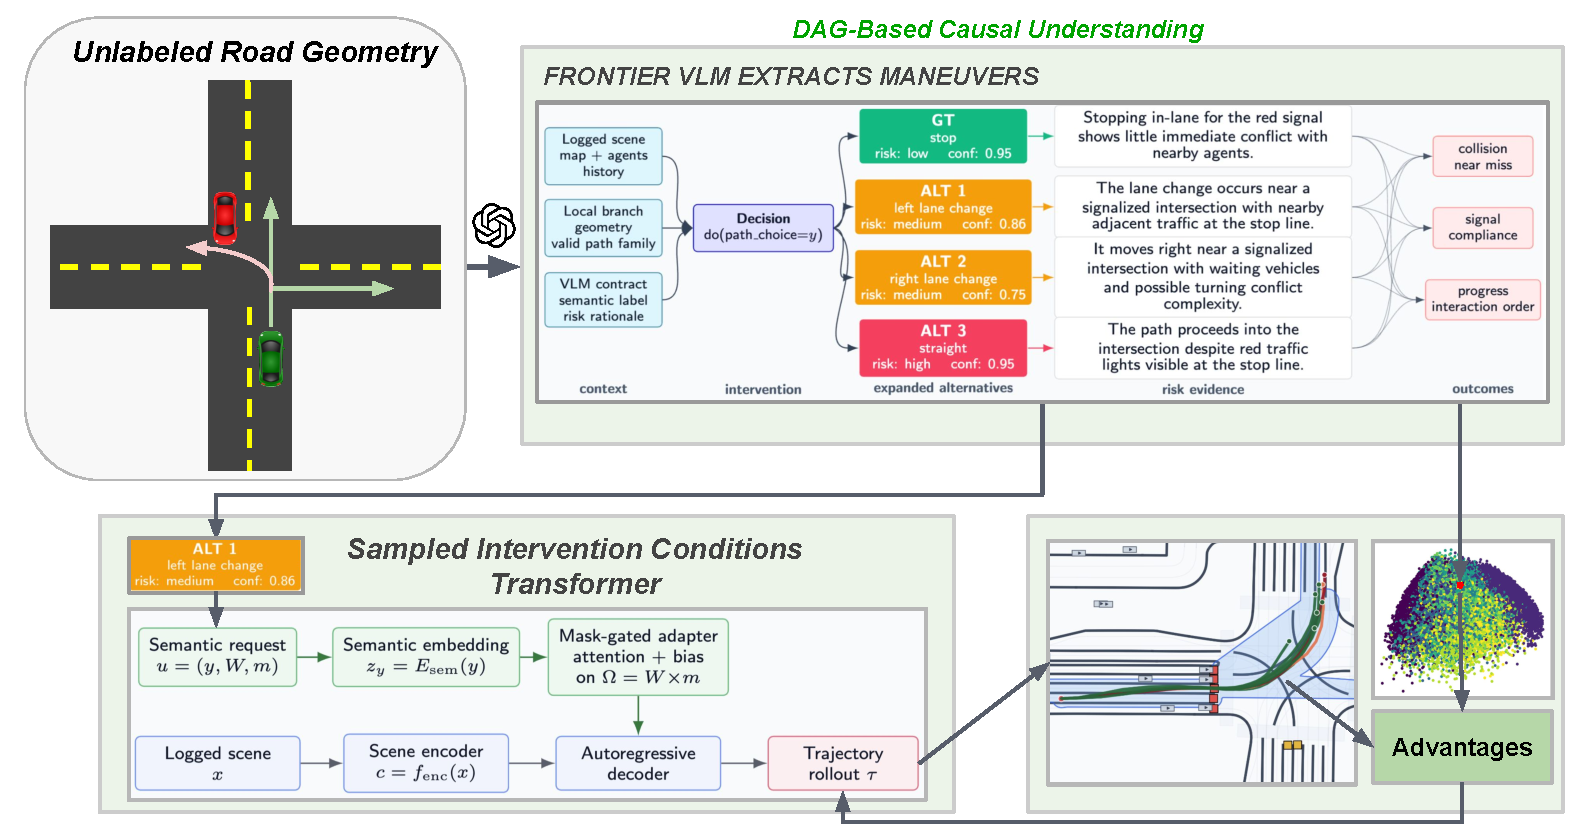
\includegraphics[width=\textwidth]{figures/CounterDriveFigure1.pdf}
  \caption{CounterDrive framework overview. A logged driving scene is converted into geometry-grounded local alternatives, organized by a sparse causal contract, and passed to a semantic-control MotionLM generator. The generated counterfactual rollouts are scored by branch validity, progress, realism, and topology-aware rollout objectives before being used for scenario generation and downstream agent training.}
  \label{fig:counterdrive-framework}
\end{figure*}

\section{Problem Setup}
\label{sec:problem-setup}

Synthetic scenario generation for autonomous driving starts from a logged scene $x$ containing a set of modeled agents $\mathcal{A}$, map context, and interaction history. The general objective is to generate alternative futures that are useful for downstream training, evaluation, or analysis while remaining plausible under the scene context. This broad setup is shared across much of the recent literature on safety-critical scenario generation. STRIVE formulates the problem as generating realistic but challenging scenarios around a real traffic scene using a learned traffic prior \citep{rempe2022strive}. CAT treats scenario generation as dynamic environment augmentation, turning log-replay scenes into safety-critical ones for closed-loop adversarial training \citep{zhang2023cat}. SEAL similarly studies closed-loop scenario perturbation, but emphasizes realistic adversarial behaviors through learned objectives and human-like skills \citep{stoler2025seal}. Adv-BMT augments real-world scenarios with diverse and realistic adversarial interactions through adversarial initialization and inverse motion reconstruction \citep{liu2025advbmt}. Across these formulations, the common goal is to expand the long tail of safety-critical behavior beyond what is directly observed in logged data.

From a counterfactual perspective, the relevant object is not an arbitrary perturbed rollout but an alternative future associated with some intervention on the scene. Let $x$ denote the observed scene and let $\tau$ denote a generated future. A counterfactual generation problem asks for plausible rollouts of the form
\[
\tau \sim p(\tau \mid x, \operatorname{do}(u)),
\]
where $u$ represents an intervention variable specifying what aspect of the scene is changed. In this view, synthetic scenario generation can be understood as choosing interventions that transform a factual logged scene into informative alternative futures while preserving as much of the original scene context as possible. The role of the intervention is to distinguish changes that are meant to be caused from changes that should remain tied to the original scene.

This framing introduces three general requirements. First, a generated future should remain \emph{plausible}: it should be dynamically and behaviorally consistent with the map, traffic configuration, and agent interaction history, as emphasized by prior methods that explicitly balance realism against difficulty \citep{rempe2022strive,stoler2025seal,liu2025advbmt}. Second, it should be \emph{intervention-consistent}: the generated future should reflect the intended change rather than an unrelated perturbation. Third, it should be \emph{scene-grounded}: the alternative future should still be recognizable as arising from the original scene rather than from an abstract adversarial objective detached from context.

These requirements are broad enough to cover both safety-critical synthetic data generation and counterfactual motion generation. They also clarify the central problem that motivates this paper: how to define interventions so that generated safety-critical futures are not only difficult or rare, but also causally meaningful with respect to the scene from which they are derived.

\section{Geometry-Grounded Counterfactual Supervision}
\label{sec:geometry-grounded-supervision}

We instantiate the general counterfactual generation problem above using scene-grounded local interventions. Given a logged scene $x$, we focus on a designated decision point for an agent $a^\star \in \mathcal{A}$ at time $t_d$. Around $(x,a^\star,t_d)$, we recover a local decision point from scene geometry and enumerate a set of locally valid alternatives
\[
\mathcal{B}(x,a^\star,t_d)=\{b_1,\dots,b_M\}.
\]
One element corresponds to the factual maneuver observed in the log, while the remaining elements correspond to geometrically valid counterfactual branches available from the same scene context. Our goal is to intervene on this local factual decision while preserving the surrounding scene and allowing downstream outcomes to change only as a consequence of that intervention.

We group branch alternatives into a compact semantic vocabulary $y \in \mathcal{Y}$, such as \texttt{left}, \texttt{right}, \texttt{straight}, \texttt{stop}, or lane-change classes. Each label denotes a \emph{family} of valid geometric realizations rather than a single exact path. A runtime control signal is represented as
\[
u=(y, W, m),
\]
where $y$ is the requested maneuver label, $W \in \{0,1\}^{T}$ is a temporal support mask, and $m \in \{0,1\}^{|\mathcal{A}|}$ is a decision-agent mask selecting which modeled agent is controlled. In the main training bank, supervision is built around the SDC. However, the control interface itself is mask-based and SDC indices are randomized, allowing for agent-agnostic intervention.

Counterfactual supervision is constructed from local lane navigation information extracted from the Waymo Open Motion Dataset v1.3.1 SDC paths field, where each path is heuristically built from scene geometry. For each candidate intervention point, we build a structured local intervention record containing the scene context, the recovered factual decision, the set of valid alternatives, supervision gates, and trainability metadata. This representation records which variable is being changed, when it is changed, and which downstream effects are permitted to vary.

A key design choice is the separation between \emph{semantic control} and \emph{geometric support}. At inference time, the model receives only the semantic request and target mask. During dataset construction and training, however, each semantic label is tied to a family of valid geometric alternatives derived from the local navigation information. A generated rollout $\tau$ is valid when it both realizes the requested semantic intervention and remains within the counterfactual support induced by the selected branch family. We therefore evaluate rollouts against a \emph{valid tube} defined by the navigation branch families rather than against a single privileged target path.

This setup is the main paper-specific instantiation of the broader problem definition in Section~\ref{sec:problem-setup}. It is what lets CounterDrive target safety-critical futures that are not only rare or difficult, but also locally interpretable, geometry-grounded, and causally meaningful.

\section{Method}
\label{sec:method}

\subsection{Causal DAG Construction}
\label{sec:causal-dag-interface}

Each local intervention is projected into a sparse causal graph.
\[
G=(V,E).
\]
We use this DAG as a semantic scaffold representing a rich intervention view. The nodes encode essential context, decisions, and outcome variables, including traffic light states, conflict timing, path choice, compliance, entry timing, stopline crossing, interaction order, and collision-related outcomes. Edges encode explicit causal hypotheses such as
\[
\texttt{signal state} \rightarrow \texttt{compliance}, \qquad
\texttt{conflict timing} \rightarrow \texttt{entry timing},
\]
and
\[
\begin{aligned}
&\{\texttt{path choice}, \texttt{compliance}, \texttt{entry timing}\} \\
&\qquad\rightarrow \{\texttt{crossing}, \texttt{collision}, \texttt{interaction order}\}.
\end{aligned}
\]

This rich scene graph is useful for scenario filtering but is too high dimensional for effective learning. At training time, we use a compactified maneuver-outcome contract sampled from the DAG that retains the decision factors most relevant to trajectory realization. This compact DAG context is encoded through maneuver-related factors such as branch, compliance, and timing, and is then used to regularize rollout behavior. This design keeps the graph representation sparse and interpretable while still providing a causal semantic anchor for downstream optimization.

\subsection{CounterDrive Architecture}
\label{sec:semantic-control}

CounterDrive builds on the Adv-BMT bidirectional motion transformer architecture \citep{liu2025advbmt}. We keep the same high-level MotionLM decomposition: a scene encoder embeds agent histories, map context, and traffic-light state, and an autoregressive motion decoder predicts future action tokens that are decoded into trajectories. This preserves the strong traffic prior learned by the pretrained Adv-BMT model while giving us a narrow place to add intervention control.

\paragraph{Backbone and token prediction.}
Let $c = f_{\mathrm{enc}}(x)$ denote the encoded scene context and let $a_{1:t-1}$ denote previously generated motion tokens. The base decoder defines
\[
\pi_{\theta}(a_t \mid x,a_{<t}) =
f_{\mathrm{dec}}(a_{<t},c).
\]
In ordinary pretraining, this model is optimized by teacher-forced cross-entropy against logged trajectories. CounterDrive retains this objective for factual reconstruction and for the \texttt{no\_intervention} control, which acts as a realism anchor.

\paragraph{Semantic-only control interface.}
At runtime, the model receives the tuple $(y,W,m)$ rather than an exact target path. The label $y$ is drawn from a compact maneuver vocabulary, including classes such as \texttt{left}, \texttt{right}, \texttt{left\_lane\_change}, \texttt{right\_lane\_change}, \texttt{straight}, \texttt{stop}, and \texttt{no\_intervention}. Let $z_y = E_{\mathrm{sem}}(y)$ denote the learned semantic embedding. The temporal-agent support of the intervention is
\[
\Omega = \{(t,n) : W_t = 1,\; m_n = 1\}.
\]
The semantic label specifies the intended maneuver family, while $W$ and $m$ specify where that intervention is allowed to act. In our current experiments the supervised bank is SDC-centered, but the interface is written as a temporal-agent mask so that the decoder API does not require exact path identifiers.

\paragraph{Local semantic adapters.}
The decoder uses the semantic request in two complementary ways. First, $z_y$ is injected as a compact maneuver memory through decoder-side attention, allowing the controlled agent to attend to the requested maneuver while still conditioning on the full traffic scene. Second, a learned local semantic residual is added only at controlled positions. Abstractly, if $h_{t,n}$ denotes the decoder state at time $t$ for agent $n$, then
\[
h'_{t,n}
=
h_{t,n}
+
\mathbf{1}[(t,n)\in\Omega]\;\Delta_{\mathrm{attn}}(h_{t,n},z_y)
+
\mathbf{1}[(t,n)\in\Omega]\;b(y),
\]
where $\Delta_{\mathrm{attn}}$ denotes the maneuver-token attention update and $b(y)$ is a learned semantic residual. The \texttt{no\_intervention} label is treated as a null semantic request: it preserves the semantic-token pathway but suppresses local intervention pressure, encouraging the model to recover factual behavior under the same control API used for counterfactual generation.

\paragraph{Trainable control modules.}
During semantic-control finetuning, most of the pretrained traffic prior can be retained while lightweight control modules are adapted: the semantic embedding table, local bias and residual gates, an auxiliary semantic prediction head, selected decoder blocks, and the output head. Counterfactual rows are shaped by family-level supervision, rollout rewards, and the topology-aware objective below, while factual or \texttt{no\_intervention} rows continue to use standard teacher-forced cross-entropy. This gives the model an explicit path back to the logged distribution while still learning to realize semantic counterfactual requests.

\subsection{Topo-MCPO Over Behavior Embeddings}
\label{sec:topo-mcpo}

The main refinement mechanism is a grouped rollout objective defined over a learned behavior space. For each scene and semantic request, we sample $K$ autoregressive futures
\[
\tau^{(1)},\dots,\tau^{(K)} \sim \pi_\theta(\cdot \mid x,u),
\]
and compute a base return $R^{(k)}$ for each rollout from branch-validity and progress-consistency signals. The important point is that optimization is not performed over isolated trajectories alone. Instead, each rollout is embedded into a behavior representation
\[
\psi_k = \Psi(\tau^{(k)}),
\]
where $\Psi$ is a learned behavior encoder operating on compact rollout features. In parallel, the intervention semantics are encoded into a compact causal context representation
\[
\phi_k = \Phi(G_k),
\]
which summarizes the maneuver-relevant DAG factors associated with the rollout.

By \emph{topology} here we mean the structure of this behavior embedding space: which rollouts lie near one another, which modes are dense or sparse, and how the sampled behaviors cluster under a fixed scene and intervention. This is the topology that drives our novelty thermostat.

\paragraph{Group-relative policy optimization.}
Within each rollout group, we compute normalized advantages
\[
\hat{A}^{(k)} = \frac{R^{(k)} - \mu_R}{\sigma_R + \varepsilon},
\]
where $\mu_R$ and $\sigma_R$ are the mean and standard deviation of returns within the sampled group. We then optimize
\[
\mathcal{L}_{\mathrm{GRPO}}
=
-
\frac{1}{K}
\sum_{k=1}^{K}
\hat{A}^{(k)}
\sum_{t=1}^{T}
\log \pi_\theta(a_t^{(k)} \mid x,u,a_{<t}^{(k)}).
\]
This makes the update relative to competing counterfactual realizations of the same scene, which is a natural fit for semantic intervention training.

\paragraph{Consensus and novelty in behavior space.}
We cluster the rollout embeddings $\{\psi_k\}_{k=1}^{K}$ using a fixed-radius rule in behavior space, producing clusters $\{C_j\}$. Let
\[
\rho_j = \frac{|C_j|}{K}
\]
denote the mass of cluster $C_j$, and let $Q_j$ denote its quality score, computed from the normalized returns of the rollouts assigned to that cluster. This yields a consensus reward
\[
c_k = \rho_{c(k)} Q_{c(k)},
\]
where $c(k)$ is the cluster containing rollout $k$. Consensus favors semantically coherent high-quality modes rather than isolated outliers.

Novelty is measured by a density model over the same behavior embedding space. Let $\hat{p}(\psi)$ denote an exponential-moving-average Gaussian density estimate over embeddings. The raw novelty score is
\[
n_k = -\log \hat{p}(\psi_k),
\]
which is standardized within the rollout group before being converted into a bonus. Intuitively, novelty encourages the policy to maintain support over underrepresented but still valid counterfactual behaviors.

\paragraph{Topology-aware thermostat.}
To prevent either collapse to a single safe mode or uncontrolled dispersion, we adapt the consensus and novelty weights according to the entropy of the cluster distribution
\[
H = -\sum_j \rho_j \log \rho_j.
\]
Given a target entropy $H^\star$, we update the consensus and novelty coefficients as
\[
\alpha = \max\!\left(0, \alpha_0 + k_\alpha (H - H^\star)\right),
\qquad
\eta = \max\!\left(0, \eta_0 + k_\eta (H^\star - H)\right).
\]
Thus, when the rollout group becomes too concentrated, novelty pressure increases; when it becomes too diffuse, consensus pressure increases. The policy is therefore regulated by the topology of the sampled behavior manifold rather than by a fixed exploration coefficient.

\paragraph{Behavior-semantic regularization.}
Finally, we regularize the behavior space so that it remains aligned with intervention semantics. The behavior embedding is trained to predict semantic label, branch, compliance, and timing factors, and it is aligned to the DAG-context embedding with
\[
\mathcal{L}_{\mathrm{align}}
=
1 - \cos\!\big(\psi_k,\phi_k\big).
\]
These auxiliary terms encourage the learned behavior manifold to remain semantically meaningful, which in turn makes novelty and consensus operate over interpretable behavioral structure rather than arbitrary latent directions.

Putting the pieces together, our final Topo-MCPO objective optimizes grouped counterfactual rollouts over a structured behavior manifold.

\section{Experiments}
\label{sec:experiments}


% Intervention example figure setup: edit the labels and filenames below.
% If a filename is empty, the panel remains a placeholder box.
\newcommand{\exampleOneTruthLabel}{Ground truth}
\newcommand{\exampleOneInterventionALabel}{left}
\newcommand{\exampleOneInterventionBLabel}{right\_lane\_change}
\newcommand{\exampleOneInterventionCLabel}{right}
\newcommand{\exampleTwoTruthLabel}{Ground truth}
\newcommand{\exampleTwoInterventionALabel}{left\_lane\_change}
\newcommand{\exampleTwoInterventionBLabel}{right\_lane\_change}
\newcommand{\exampleTwoInterventionCLabel}{right}
\newcommand{\exampleOneTruthFile}{figures/8_gt.png}
\newcommand{\exampleOneInterventionAFile}{figures/8_left.png}
\newcommand{\exampleOneInterventionBFile}{figures/8_lane.png}
\newcommand{\exampleOneInterventionCFile}{figures/8_right.png}
\newcommand{\exampleTwoTruthFile}{figures/79_gt.png}
\newcommand{\exampleTwoInterventionAFile}{figures/79_left_lane.png}
\newcommand{\exampleTwoInterventionBFile}{figures/79_right_lane.png}
\newcommand{\exampleTwoInterventionCFile}{figures/79_right.png}
\newcommand{\interventionexampleslot}[2]{%
  \begingroup
  \edef\interventionexamplefile{#1}%
  \ifx\interventionexamplefile\empty
    \fbox{\parbox[c][1.25in][c]{0.95\linewidth}{\centering\footnotesize #2\\[0.35em]Add image filename above}}%
  \else
    \includegraphics[width=\linewidth]{#1}%
  \fi
  \endgroup
}
\newcommand{\interventionexamplecell}[3]{%
  \begin{minipage}[t]{0.23\textwidth}
    \centering
    \textbf{#1}\\[0.35em]
    \interventionexampleslot{#2}{#3}
  \end{minipage}%
}

\begin{figure*}[t]
  \centering
  \interventionexamplecell{\exampleOneTruthLabel}{\exampleOneTruthFile}{}
  \hfill
  \interventionexamplecell{\exampleOneInterventionALabel}{\exampleOneInterventionAFile}{Example 1 intervention A}
  \hfill
  \interventionexamplecell{\exampleOneInterventionBLabel}{\exampleOneInterventionBFile}{Example 1 intervention B}
  \hfill
  \interventionexamplecell{\exampleOneInterventionCLabel}{\exampleOneInterventionCFile}{Example 1 intervention C}

  \vspace{0.9em}

  \interventionexamplecell{\exampleTwoTruthLabel}{\exampleTwoTruthFile}{Example 2 ground truth}
  \hfill
  \interventionexamplecell{\exampleTwoInterventionALabel}{\exampleTwoInterventionAFile}{Example 2 intervention A}
  \hfill
  \interventionexamplecell{\exampleTwoInterventionBLabel}{\exampleTwoInterventionBFile}{Example 2 intervention B}
  \hfill
  \interventionexamplecell{\exampleTwoInterventionCLabel}{\exampleTwoInterventionCFile}{Example 2 intervention C}
  \caption{Example CounterDrive interventions. Each row corresponds to one logged scene. The left column shows the ground-truth trajectory, and the three right columns show counterfactual interventions.}
  \label{fig:intervention-examples}
\end{figure*}

\subsection{Experimental Setup}
\label{sec:experimental-setup}
We evaluate CounterDrive on WOMD/Waymax-derived ScenarioNet scenes. For each logged scene, preprocessing enumerates SDC branch alternatives from local navigation paths, removes degenerate or ambiguous targets, and stores one control row per factual or counterfactual semantic request. Unless otherwise stated, generation uses the trained CounterDrive semantic-control model and samples autoregressive futures conditioned only on the requested maneuver label and target mask. We report two generation settings: an all-label setting, where every valid semantic branch is generated to measure coverage and diversity, and a GT-aligned setting, where the requested label matches the logged maneuver so that displacement realism metrics are meaningful.

We evaluate generated scenarios along two axes. First, we measure open-loop realism and diversity using SADE/SFDE, min-SADE/min-SFDE, velocity and TTC JSD, and ADD/FDD. Second, we convert generated scenarios into ScenarioNet views for downstream TD3 training. Downstream comparisons use Waymo-only, Adv-BMT-augmented, and CounterDrive-augmented training sets, with augmented data constructed at a 1:1 ratio between logged and generated scenes. Evaluation reports reward, step cost, route completion, collision rate, and episode cost sum on held-out Waymo validation scenes. For ablations, we keep the data and evaluation code fixed while changing only the rollout objective or the risk tier used to select synthetic scenes.

\subsection{Scenario Realism and Diversity}
\label{sec:scenario-realism-diversity}
Before evaluating downstream policy learning, we first evaluate the quality of the generated CounterDrive scenarios themselves. In our setting, we report two complementary evaluations. \emph{CounterDrive (ours)} uses trajectories generated from all enumerated guidance labels for each scene, which is the relevant setting for measuring coverage and behavioral diversity. \emph{CounterDrive (ours) GT} evaluates only the subset of scenes where the selected guidance matches the ground-truth maneuver, which makes direct realism comparisons possible using displacement-based forecasting metrics. This separation is important because GT-aligned accuracy metrics such as SADE and SFDE are not meaningful when a scene is intentionally expanded into multiple non-factual counterfactual branches.

Accordingly, Table~\ref{tab:counterdrive-realism-diversity} reports realism on the GT-only split using SADE, min-SADE, SFDE, min-SFDE, and JSD-based distributional metrics over velocity and time-to-collision. It then reports all-label diversity using ADD and FDD, which capture how broadly the framework explores distinct counterfactual outcomes. We restrict this table to methods for which we can run the same local GT/all-label evaluation protocol, while broader downstream comparisons to CAT~\citep{zhang2023cat}, SEAL~\citep{stoler2025seal}, and STRIVE~\citep{rempe2022strive} are reported separately in Figure~\ref{fig:downstream-procedure-comparison}.

\begin{table*}[t]
\centering
\small
\setlength{\tabcolsep}{5pt}
\renewcommand{\arraystretch}{1.08}
\caption{Realism and diversity of generated CounterDrive scenarios. \textbf{CounterDrive (ours)} is evaluated on trajectories generated from all enumerated guidance labels for each scene, while \textbf{CounterDrive (ours) GT} is evaluated on the subset where guidance matches the ground-truth maneuver. Realism metrics are reported on the GT-only split; diversity metrics are reported on the full all-label split. Lower is better for realism metrics, and higher is better for diversity metrics.}
\label{tab:counterdrive-realism-diversity}
\resizebox{\textwidth}{!}{%
\begin{tabular}{@{}lcccccccc@{}}
\toprule
& \multicolumn{6}{c}{\textit{Realism on GT-only split}} & \multicolumn{2}{c}{\textit{All-label diversity}} \\
\cmidrule(lr){2-7} \cmidrule(lr){8-9}
\textbf{Method} & SADE $\downarrow$ & min-SADE $\downarrow$ & SFDE $\downarrow$ & min-SFDE $\downarrow$ & Vel-JSD $\downarrow$ & TTC-JSD $\downarrow$ & ADD $\uparrow$ & FDD $\uparrow$ \\
\midrule
Adv-BMT & 0.90 & 0.32 & 4.26 & \textbf{1.47} & 0.23 & 0.30 & 4.77 & 11.44 \\
\textbf{CounterDrive (ours)} & -- & -- & -- & -- & 0.24 & 0.27 & \textbf{40.42} & \textbf{87.46} \\
\textbf{CounterDrive (ours) GT} & \textbf{0.84} & \textbf{0.22} & \textbf{2.77} & 2.01 & \textbf{0.20} & \textbf{0.26} & -- & -- \\
\bottomrule
\end{tabular}%
}
\end{table*}

\subsection{Main Results}
\label{sec:main-results}
To measure whether CounterDrive scenarios improve downstream agent learning, we follow an open-loop policy-training protocol~\citep{liu2025advbmt} and adapt it to our setting. For the primary head-to-head comparison in Table~\ref{tab:counterdrive-open-loop}, we only include methods for which we can evaluate on the same local validation scenes: Waymo-only training, Adv-BMT augmentation, and CounterDrive augmentation. This is due to both a lack of availibility for some of the models as well as computational constraints. Starting from the logged training split, each augmented setting pairs real scenes with generated safety-critical scenarios, yielding a 1:1 ratio between logged and generated data.

For the downstream RL agent evaluation task we report average reward, average step cost, route completion rate, collision rate, and episode cost sum. This experiment is the main downstream validation of the dataset itself: the central question is whether agents trained with CounterDrive-generated scenarios become stronger in end-to-end comparison. Table~\ref{tab:counterdrive-open-loop} provides the primary same-split summary. For broader context, Figure~\ref{fig:downstream-procedure-comparison} compares CounterDrive against published baselines under a procedure-consistent evaluation: we use the same random-100 selection process used in Adv-BMT \cite{liu2025advbmt} and report the resulting CounterDrive mean and standard deviation over 10 evaluations.

\begin{table*}[t]
  \centering
  \caption{Open-loop downstream agent evaluation with CounterDrive-generated scenarios. Each logged scenario is augmented with one generated safety-critical scenario, so the ratio between real-world and generated scenes is 1:1. For each method, we train the same downstream agent on the corresponding augmented dataset and report the mean.}
  \label{tab:counterdrive-open-loop}
  \small
  \begin{tabular}{lcccc}
    \toprule
    \multicolumn{5}{c}{(a) Evaluation on original validation environments} \\
    \midrule
    Training scenarios & Reward $\uparrow$ & Cost $\downarrow$ & Completion $\uparrow$ & Collision $\downarrow$ \\
    \midrule
    Waymo only & 48.7 & 0.35 & 0.741 & 0.01 \\
    Adv-BMT & 32.7 & 0.56 & 0.603 & 0.04 \\
    \textbf{CounterDrive (ours)} & 51 & 0.32 & 0.806 & 0.03 \\
    \bottomrule
  \end{tabular}
  \iffalse
  \vspace{0.75em}

  \begin{tabular}{lccccc}
    \toprule
    \multicolumn{6}{c}{(b) Evaluation on CounterDrive validation environments} \\
    \midrule
    Training scenarios & Reward $\uparrow$ & Cost $\downarrow$ & Completion $\uparrow$ & Collision $\downarrow$ & Cost sum $\downarrow$ \\
    \midrule
    Waymo only & -- & -- & -- & -- & -- \\
    Adv-BMT & -- & -- & -- & -- & -- \\
    \textbf{CounterDrive (ours)} & -- & -- & -- & -- & -- \\
    \bottomrule
  \end{tabular}
  \fi
\end{table*}

\begin{figure*}[t]
  \centering
  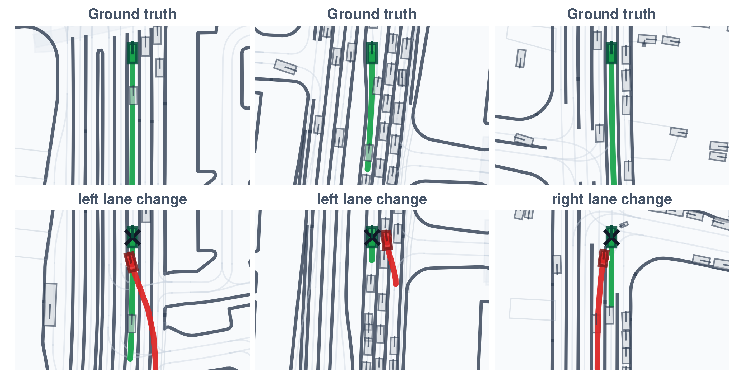
\includegraphics[width=\textwidth]{figures/adversarial_counterfactual_three_scenarios.pdf}
  \caption{Qualitative adversarial CounterDrive examples. Each column shows one logged scene. The top row shows the factual playback, and the bottom row shows the corresponding adversarial counterfactual produced by applying a semantic maneuver intervention to a nearby non-SDC agent. Green marks the SDC trajectory and red marks the intervened adversary.}
  \label{fig:adversarial-counterfactual-examples}
\end{figure*}

\begin{table}[t]
  \centering
  \small
  \setlength{\tabcolsep}{6pt}
  \renewcommand{\arraystretch}{1.05}
  \caption{Scenario-level SDC--adversary crash rates for generated counterfactual scenes.}
  \label{tab:generated-crash-rates}
  \begin{tabular}{lccc}
    \toprule
    Method & Scenes & Contact (\%) & Close Collision (\%) \\
    \midrule
    CAT & 497 & 50.7 & 67.8 \\
    STRIVE & 484 & 33.9 & 46.9 \\
    SEAL & 360 & 59.2 & 72.2 \\
    Adv-BMT & 476 & 100.0 & 100.0 \\
    \textbf{CounterDrive (ours)} & 476 & 44.7 & 70.4 \\
    \bottomrule
  \end{tabular}
\end{table}

\begin{figure*}[t]
  \centering
  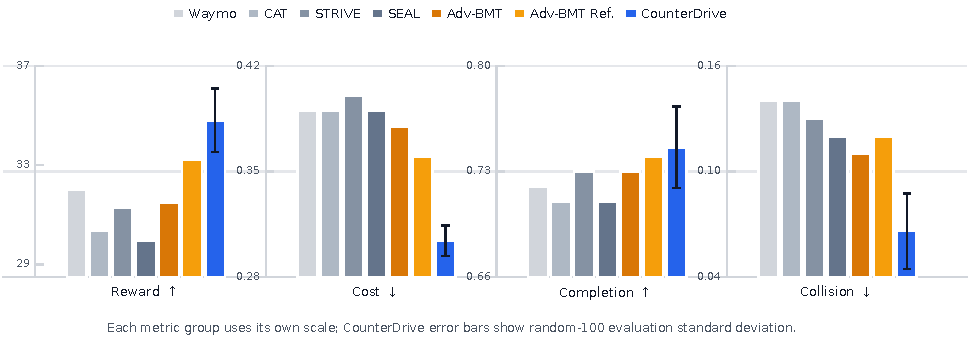
\includegraphics[width=\textwidth]{figures/downstream_procedure_comparison.pdf}
  \caption{Downstream comparison to the baselines Adv-BMT~\citep{liu2025advbmt}, SEAL~\citep{stoler2025seal}, CAT~\citep{zhang2023cat}, and STRIVE~\citep{rempe2022strive}. Baseline bars use the published Waymo-validation means while CounterDrive reports our repeated random-100 evaluation mean with standard deviation. Bars are grouped by metric.}
  \label{fig:downstream-procedure-comparison}
\end{figure*}

\subsection{Ablations and Analysis}
\label{sec:ablations}
We include two focused ablation families to isolate where the gains in CounterDrive come from. The first compares topology-aware policy optimization against a GRPO rollout baseline. The second studies how the estimated safety-criticality of synthetic scenarios affects downstream agent learning. Together, these ablations help separate the value of the optimization method from the value of the generated data distribution.

\subsubsection{Topo-MCPO versus GRPO rollout training}
We compare the full topology-aware optimization procedure against a matched GRPO baseline using the same backbone, counterfactual dataset, and all-label evaluation protocol. This ablation is designed to answer whether topology-aware rollout structure improves intervention quality beyond group-relative optimization alone. Because all-label evaluation intentionally requests non-factual semantic alternatives, displacement to the logged future should not be interpreted as ordinary forecasting accuracy. Instead, all-agent ADE and FDE act as scene-proximity diagnostics: lower values indicate that generated interventions preserve more of the original scene context while still changing the controlled decision.

\begin{figure*}[t]
  \centering
  \begin{minipage}[t]{0.49\textwidth}
    \centering
    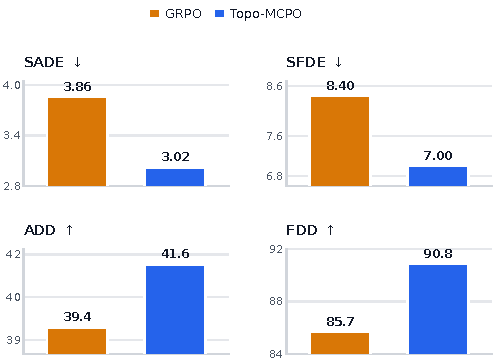
\includegraphics[width=\linewidth]{figures/topomcpo_vs_grpo_ablation.pdf}
    \vspace{-1.2em}
    \caption{Topo-MCPO versus GRPO under all-label evaluation.}
    \label{fig:topomcpo-vs-grpo}
  \end{minipage}
  \hfill
  \begin{minipage}[t]{0.49\textwidth}
    \centering
    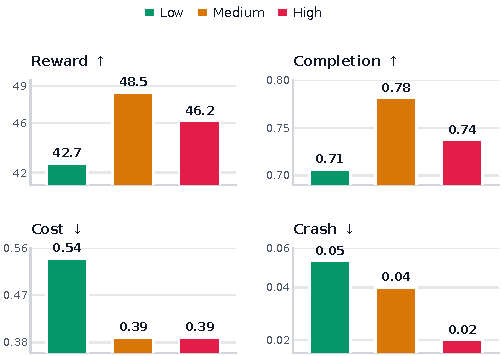
\includegraphics[width=\linewidth]{figures/risk_ablation_4panel.pdf}
    \vspace{-1.2em}
    \caption{Downstream ablation by synthetic scenario risk tier.}
    \label{fig:risk-level-ablation}
  \end{minipage}
\end{figure*}

Figure~\ref{fig:topomcpo-vs-grpo} shows that Topo-MCPO reduces all-agent SADE from 3.86 to 3.02 and all-agent SFDE from 8.40 to 7.00 relative to GRPO. At the same time, scene-level semantic ADD increases from 39.44 to 41.65 and scene-level semantic FDD increases from 85.68 to 90.84. We therefore interpret the result as a paired realism-and-coverage improvement under the same intervention protocol: Topo-MCPO stays closer to the ground-truth scene context while producing broader semantic variation.

\subsubsection{Effect of safety-critical scenario rating}
We also study how partitioning scenes by the risk assigned by the causal DAG affects the quality of learned agents. We partition generated scenarios by assessed safety-criticality: low-risk, medium-risk, and high-risk, then train otherwise identical agents on each subset. This ablation is intended to measure whether VLM risk assessment is an effective signal for training data quality, whether high-risk-only training hurts nominal driving performance, and whether a balanced mixture is preferable to any single risk band.

\section{Discussion}
\label{sec:discussion}
\paragraph{Counterfactual scenario generation from real logs.}
CounterDrive is motivated by the observation that a logged driving scene contains more information than its single observed future. The factual trajectory records one realized decision, but the map geometry, lane connectivity, traffic state, and nearby agents often imply a set of plausible alternatives. Our results suggest that treating these alternatives as structured counterfactual interventions is a useful way to expand safety-critical data without abandoning the realism of the original log. The GT-aligned realism evaluation shows that the generator can remain close to factual behavior when the semantic request agrees with the log, while the all-label evaluation shows much larger ADD and FDD than the Adv-BMT baseline. This is the intended behavior: the model should preserve scene context when asked to reconstruct the factual branch, but it should not collapse to the factual branch when asked to realize a valid alternative.

A central design choice is to supervise semantic families rather than exact paths. This matters because an intervention such as \texttt{left\_lane\_change} or \texttt{right} is not a single polyline; it is a class of geometrically valid realizations with different speeds, timings, and interaction outcomes. Exact-path conditioning would make the control interface easier to evaluate but less useful as a scenario generator, because it would move the burden of specifying the full future trajectory back to the user. CounterDrive instead exposes a compact semantic request at inference time and uses privileged branch-family information only during construction, training, and scoring. This separation helps explain why the method can improve diversity while retaining competitive realism; the generator is constrained by a valid region, not just a single target path.


\paragraph{Downstream applications.}
The downstream experiments indicate that CounterDrive scenarios can improve policy training while preserving nominal performance. In the same-split evaluation, training with CounterDrive-generated scenarios improves reward and completion relative to the Waymo-only setting, while maintaining moderate cost and collision rates. In comparison with Adv-BMT-style augmentation, CounterDrive performs better on reward and completion in our local evaluation. These results support the view that semantic counterfactuals are useful not only as qualitative examples or stress tests, but also as training data for downstream agents.

The ablations clarify where this utility comes from. Topo-MCPO improves both scene-proximity diagnostics and semantic coverage relative to the matched GRPO rollout baseline. This suggests that the behavior-space structure is doing useful work; group-relative optimization alone can reward high-return samples, but the topology-aware terms help regulate the distribution of generated behaviors. The novelty and consensus components are especially relevant for counterfactual generation, where a generator that produces only one high-probability safe mode is insufficient, but a generator that disperses into unrealistic branches is also undesirable. The thermostat mechanism provides a way to tune this tradeoff from the sampled rollout group itself.

The risk ablation points to a complementary use of the DAG and VLM-derived contracts. Risk labels are not used merely as descriptive annotations; they can organize synthetic training data into subsets with different downstream effects. This provides a practical pathway for curriculum design and dataset construction. In deployment-oriented settings, one may prefer a balanced mixture that improves robustness without overfitting the agent to extreme cases. In evaluation-oriented settings, higher-risk subsets may be useful for targeted stress testing. CounterDrive naturally supports both uses because the generated scenarios remain linked to explicit intervention and risk contracts.

%\paragraph{Scientific takeaway.}
%The main takeaway is that controllable scenario generation benefits from %aligning three levels of structure: geometry, semantics, and optimization. %Geometry supplies the local alternatives and valid regions; semantics gives %a compact intervention interface; rollout optimization encourages the model %to realize the request while preserving plausible traffic behavior. None of %these pieces alone is sufficient. Geometry without semantic control %produces path-specific supervision rather than a usable intervention %interface. Semantic labels without valid regions are too weak to define %whether a rollout actually realizes the intended counterfactual. Rollout RL %without a structured behavior space can improve reward while reducing %realism or diversity. CounterDrive combines these elements into a single %training and evaluation pipeline.

There are also limitations. The current intervention bank is built primarily around SDC-centered branches, and the semantic labels depend on the quality of the local path enumeration and VLM-assisted labeling. The \texttt{no\_intervention} and factual-CE repair experiments further show that realism can depend sensitively on the mixture between factual anchoring and counterfactual optimization. These limitations do not change the central empirical findings, but they identify the next steps: stronger agent-agnostic intervention banks, better calibrated semantic labeling, and a wider gamut of multi-turn interventions.

Overall, CounterDrive reframes safety-critical scenario generation as causal semantic control rather than unconstrained adversarial perturbation. This makes the generated data easier to interpret, easier to filter by risk and intervention type, and more directly connected to downstream learning objectives. The broader implication is that logged driving data can support a richer counterfactual training signal when the generator is given the right structural constraints, not just what happened, but which plausible local decisions could have happened instead, and how those decisions propagate through the scene.

\section{Related Work}
\label{sec:related-work}
\paragraph{Counterfactual and controllable motion generation.}
Recent work on safety-critical scenario generation has shown that training and evaluation benefit from augmenting logged traffic with challenging interactions rather than relying on rare events to appear naturally. STRIVE learns a traffic prior and optimizes accident-prone scenarios around existing traffic participants \citep{rempe2022strive}. In that sense, STRIVE is representative of approaches that seek realistic but planner-challenging scenarios through adversarial optimization. Our method differs in that we do not organize generation around inducing planner failure or collision directly. Instead, we define scene-grounded semantic interventions tied to natural local decision alternatives and generate counterfactual outcomes that are causally coherent with the original scene. CAT shifts the focus to closed-loop adversarial training, where the ego policy is trained against learned adversaries in simulation \citep{zhang2023cat}. SEAL introduces skill-enabled adversary learning for closed-loop scenario generation, emphasizing reusable adversarial behaviors for safe autonomous driving evaluation \citep{stoler2025seal}. Most closely related to our work, Adv-BMT uses adversarial initialization together with bidirectional motion prediction to generate realistic safety-critical traffic scenarios from real logs \citep{liu2025advbmt}. These methods establish the value of synthetic safety-critical data, but they are primarily organized around adversarial collision generation. Our setting instead emphasizes semantically specified counterfactual interventions, where the objective is not only to create a dangerous pathological interaction, but to realize a plausible alternative branch based on actual traffic and scenario context.

\paragraph{Causal structure for autonomy.}
A second line of work seeks more structured representations of why outcomes change under intervention. In many existing scenario-generation pipelines, the latent control variables behind a generated outcome remain implicit; a method may produce a collision, lane change, or evasive maneuver without explicitly modeling which local decision was changed and which downstream consequences should remain invariant. Our use of sparse causal DAGs is intended to make this interface explicit. Rather than treating generated trajectories as standalone samples, we represent counterfactual scenarios through decision-to-outcome structure, which helps distinguish scene context, intervention choice, and downstream effects. This complements prior scenario-generation baselines by adding a causal semantic scaffold on top of geometric and behavioral generation.

\paragraph{Structured behavior spaces and geometry-aware rollout optimization.}
Recent multi-agent traffic generation and motion-modeling work increasingly treats behavior as a structured object rather than a single best-fit trajectory. The baselines above already move in this direction in different ways: STRIVE uses a learned traffic prior \citep{rempe2022strive}, CAT optimizes relative to a closed-loop adversary \citep{zhang2023cat}, SEAL introduces reusable adversarial skills \citep{stoler2025seal}, and Adv-BMT couples adversarial initialization with motion-model-based reconstruction of realistic interactions \citep{liu2025advbmt}. Our approach builds on this trend but focuses on geometry-aware rollout optimization for counterfactual branches. Instead of asking the model to imitate one exact target path, we score generated rollouts against valid counterfactual regions, topology-aware progress signals, and family-consistent semantic behavior structure. This positions CounterDrive as a bridge between controllable motion generation, scenario augmentation, and structured policy optimization over semantically meaningful alternative futures.


\section{Conclusion}
\label{sec:conclusion}
CounterDrive addresses the scarcity of safety-critical driving data by treating logged scenes as sources of structured counterfactual alternatives rather than fixed demonstrations. The central idea is to intervene at the level of local semantic decisions while grounding those interventions in the branch geometry of the original scene. This produces supervision that is neither arbitrary trajectory relabeling nor unconstrained adversarial perturbation. Each generated future is tied to a valid maneuver family, a target agent and time support, and an explicit account of which downstream outcomes may change.

Building on this representation, CounterDrive introduces behavioral control to an autoregressive motion generator and optimizes rollouts against counterfactual regions instead of overly constrained privileged paths. Our experiments indicate that this structure can generate diverse, realistic alternatives and produce scenarios that are useful for downstream policy training. More broadly, the results suggest that the long tail in driving can be approached by recovering the decisions a scene could have supported, generating plausible futures under explicit intervention contracts, and evaluating those futures as training data. This moves safety-critical scenario generation toward outputs that are not only challenging, but also interpretable and causally connected to the original scene.


\bibliographystyle{plainnat}
\bibliography{references}

\appendix

\section{Appendix}
\label{sec:appendix}
\begin{itemize}
  \item Full intervention contract and DAG schema.
  \item Dataset construction details, filtering rules, and split statistics.
  \item Reward definition, progress-trace construction, and failure cases of naive progress.
  \item Additional rollout visualizations and qualitative counterfactual case studies.
  \item Hyperparameters, training details, and reproducibility notes.
\end{itemize}

\newpage
\input{checklist.tex}

\end{document}
